\documentclass[a4paper, 12pt]{article}
\usepackage[T2A]{fontenc}
\usepackage[utf8]{inputenc}
\usepackage[english,russian]{babel}
\usepackage{amsmath, amsfonts, amssymb, amsthm, mathtools, misccorr, indentfirst, multirow}
\usepackage{wrapfig}
\usepackage{graphicx}
\usepackage{subfig}
\usepackage{adjustbox}
\usepackage{pgfplots}
\usepackage{mathrsfs}

\usepackage{geometry}
\geometry{top=20mm}
\geometry{bottom=20mm}
\geometry{left=20mm}
\geometry{right=20mm}
\newcommand{\angstrom}{\textup{\AA}}

\begin{document}
    \title{Влияние параметров периодического потенциала на спектр состояний и на возникновение запрещенной зоны в модели Кронига-Пенни}
    \author{Нехаев Александр 654 гр.}
    \maketitle
    \section{Периодическая задача}
    Рассмотрим одномерную решетку ионов, расстояние между которыми $a$. Потенциал при этом будет периодическим, его вид приведен на рис. \ref{fig:one}.
    \begin{figure}[h]
        \centering
        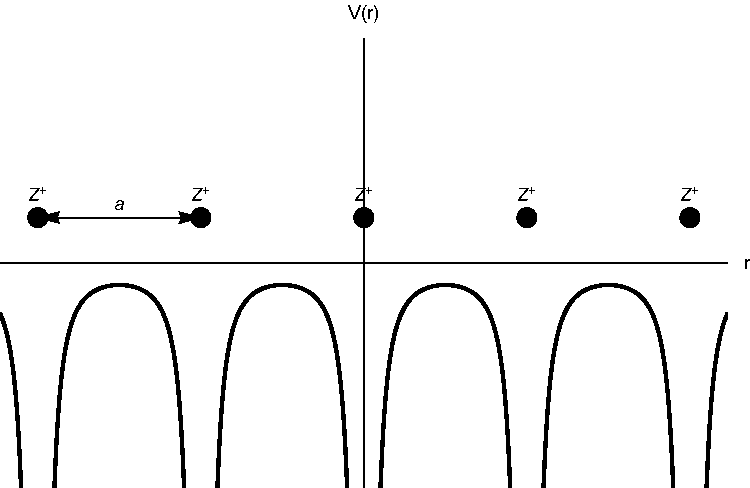
\includegraphics{fig1.pdf}
        \caption{Пример периодического потенциала}
        \label{fig:one}
    \end{figure}

    Рассмотрим идеализированный случай бесконечного кристалла. Уравнение Шрёдингера имеет вид:
    \begin{equation}
        -\frac{\hbar^2}{2m}\frac{\partial^2\psi(x)}{\partial x^2}+V_a(x)\psi(x)=E\psi(x)
    \end{equation}
    с периодическим потенциалом $V_a(x)=V_a(x+a)$. Спектр определяется как множество тех энергий, при которых уравнение имеет решения, ограниченные на всей вещественной оси.
    \section{Теорема Блоха}
    Собственные состояния одноэлектронного гамильтониана
    \begin{equation}
        \hat{H}=-\frac{\hbar^2}{2m}\nabla^2+V(\bf{r}),
    \end{equation}
    где потенциал $V(\bf{r})$ периодичен по всем векторам $\bf{R}$ решетки Бравэ, могут быть выбраны таким образом, чтобы их волновые функции имели форму плоской волны, умноженной на функцию, обладающую той же периодичностью, то и решетка Бравэ:
    \begin{equation}
        \psi_{n\bf{k}}=e^{i\bf{kr}}u_{n\bf{k}}(\bf{r}),
    \end{equation}
    где $u_{n\bf{k}}({\bf{r}+\bf{R}})=u_{n\bf{k}}(\bf{r})$, для всех $\bf{R}$, принадлежащих решетке Бравэ. Электронные волновые функции в виде $u_{n\bf{k}}({\bf{r}})=u_{n{\bf{k}}}(\bf{r+R})$ называют функциями Блоха.
    \section{Модель Кронига-Пенни}
    Для упрощения задачи потенциал приближают прямоугольным, используя теорему Блоха (рис. \ref{fig:two}).
    \begin{figure}[h]
        \centering
        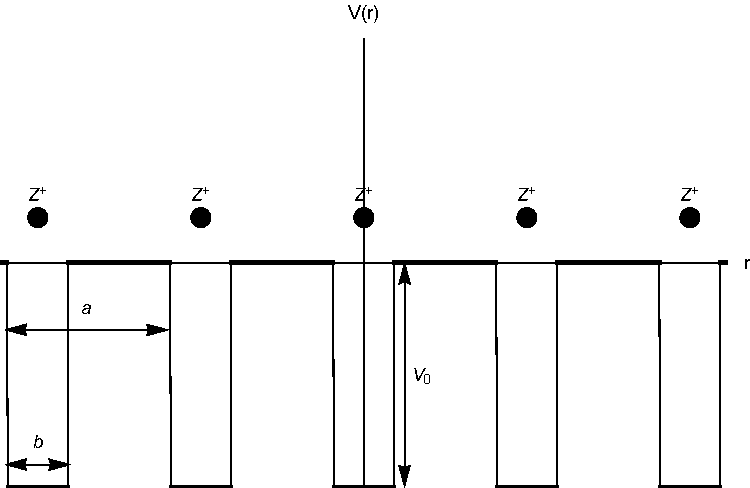
\includegraphics{fig2.pdf}
        \caption{Периодический потенциал с периодом $a$ и шириной прямоугольной ямы $b$}
        \label{fig:two}
    \end{figure}

    Распишем уравнения для двух участков: $0<x<a-b$ и $-b<x<0$:
    \begin{equation}
        \frac{-\hbar^2}{2m}\psi''=E\psi
    \end{equation}
    \begin{equation}
        \frac{-\hbar^2}{2m}\psi''=(E+V_0)\psi
    \end{equation}
    При их решении получаем для волновой функции "на поверхности":
    \begin{equation}
        \psi=Ae^{i\alpha x}+A'e^{-i\alpha x},
    \end{equation}
    где $\alpha^2=\frac{2mE}{\hbar^2}$, $A=\frac{C_1}{2}-\frac{iC_2}{2}$ и $A'=\frac{C_1}{2}+\frac{iC_2}{2}$, а для волновой функции в яме:
    \begin{equation}
        \psi=Be^{i\beta x}+B'e^{-i\beta x},
    \end{equation}
    где $\beta^2=\frac{2m(E+V_0)}{\hbar^2}$. С помощью полученных волновых функций получим соотвествующие им функции Блоха:
    \begin{equation}
        \begin{aligned}
            u(0<x<a-b)=Ae^{i(\alpha-k)x}+A'e^{-i(\alpha+k)x}\\
            u(-b<x<0)=Be^{i(\beta-k)x}+B'e^{-i(\beta+k)x}.
        \end{aligned}
    \end{equation}
    Далее проводим сшивку:
    \begin{equation}
        \begin{aligned}
            \psi(0^-)=\psi(0^+)\\
            \psi'(0^-)=\psi'(0^+)
        \end{aligned}
    \end{equation}
    и накладываем условие на периодичность функций Блоха:
    \begin{equation}
        \begin{aligned}
            u(-b)=u(a-b)\\
            u'(-b)=u'(a-b).
        \end{aligned}
    \end{equation}
    Эти условия дают матрицу:
    \begin{equation*}
        \left(
        \begin{matrix}
            1 & 1 & -1 & -1\\
            \alpha & -\alpha & -\beta & \beta \\
            e^{i(\alpha-k)(\alpha-b)} & e^{-i(\alpha+k)(a-b)} & -e^{-i(\beta-k)b} & -e^{i(\beta+k)b}\\
            (\alpha - k)e^{i(\alpha-k)(a-b)} & -(\alpha+k)e^{-i(\alpha+k)(a-b)} & -(\beta-k)e^{-i(\beta-k)b} & (\beta+k)e^{i(\beta+k)b}
        \end{matrix}
        \right)
        \left(
        \begin{matrix}
            A\\
            A'\\
            B\\
            B'
        \end{matrix}    
        \right)=
        \left(
        \begin{matrix}
            0\\
            0\\
            0\\
            0
        \end{matrix}    
        \right).
    \end{equation*}
    Необходимое условие существования нетривиального решения -- зануление детерминанта. После преобразований получаем:
    \begin{equation}
        \cos(ka)=\cos(\beta b)\cos[\alpha(a-b)]-\frac{\alpha^2+\beta^2}{2\alpha\beta}\sin(\beta b)\sin[\alpha(a-b)].
    \end{equation}
    \section{Моделирование}
    Используя методы компьютерного моделирования, была созданна программа, демонстрирующую завимость разрешенных значений энергии от параметров модели. Так же видна запрещенная зона.
    \begin{figure}[!h]
        \centering
        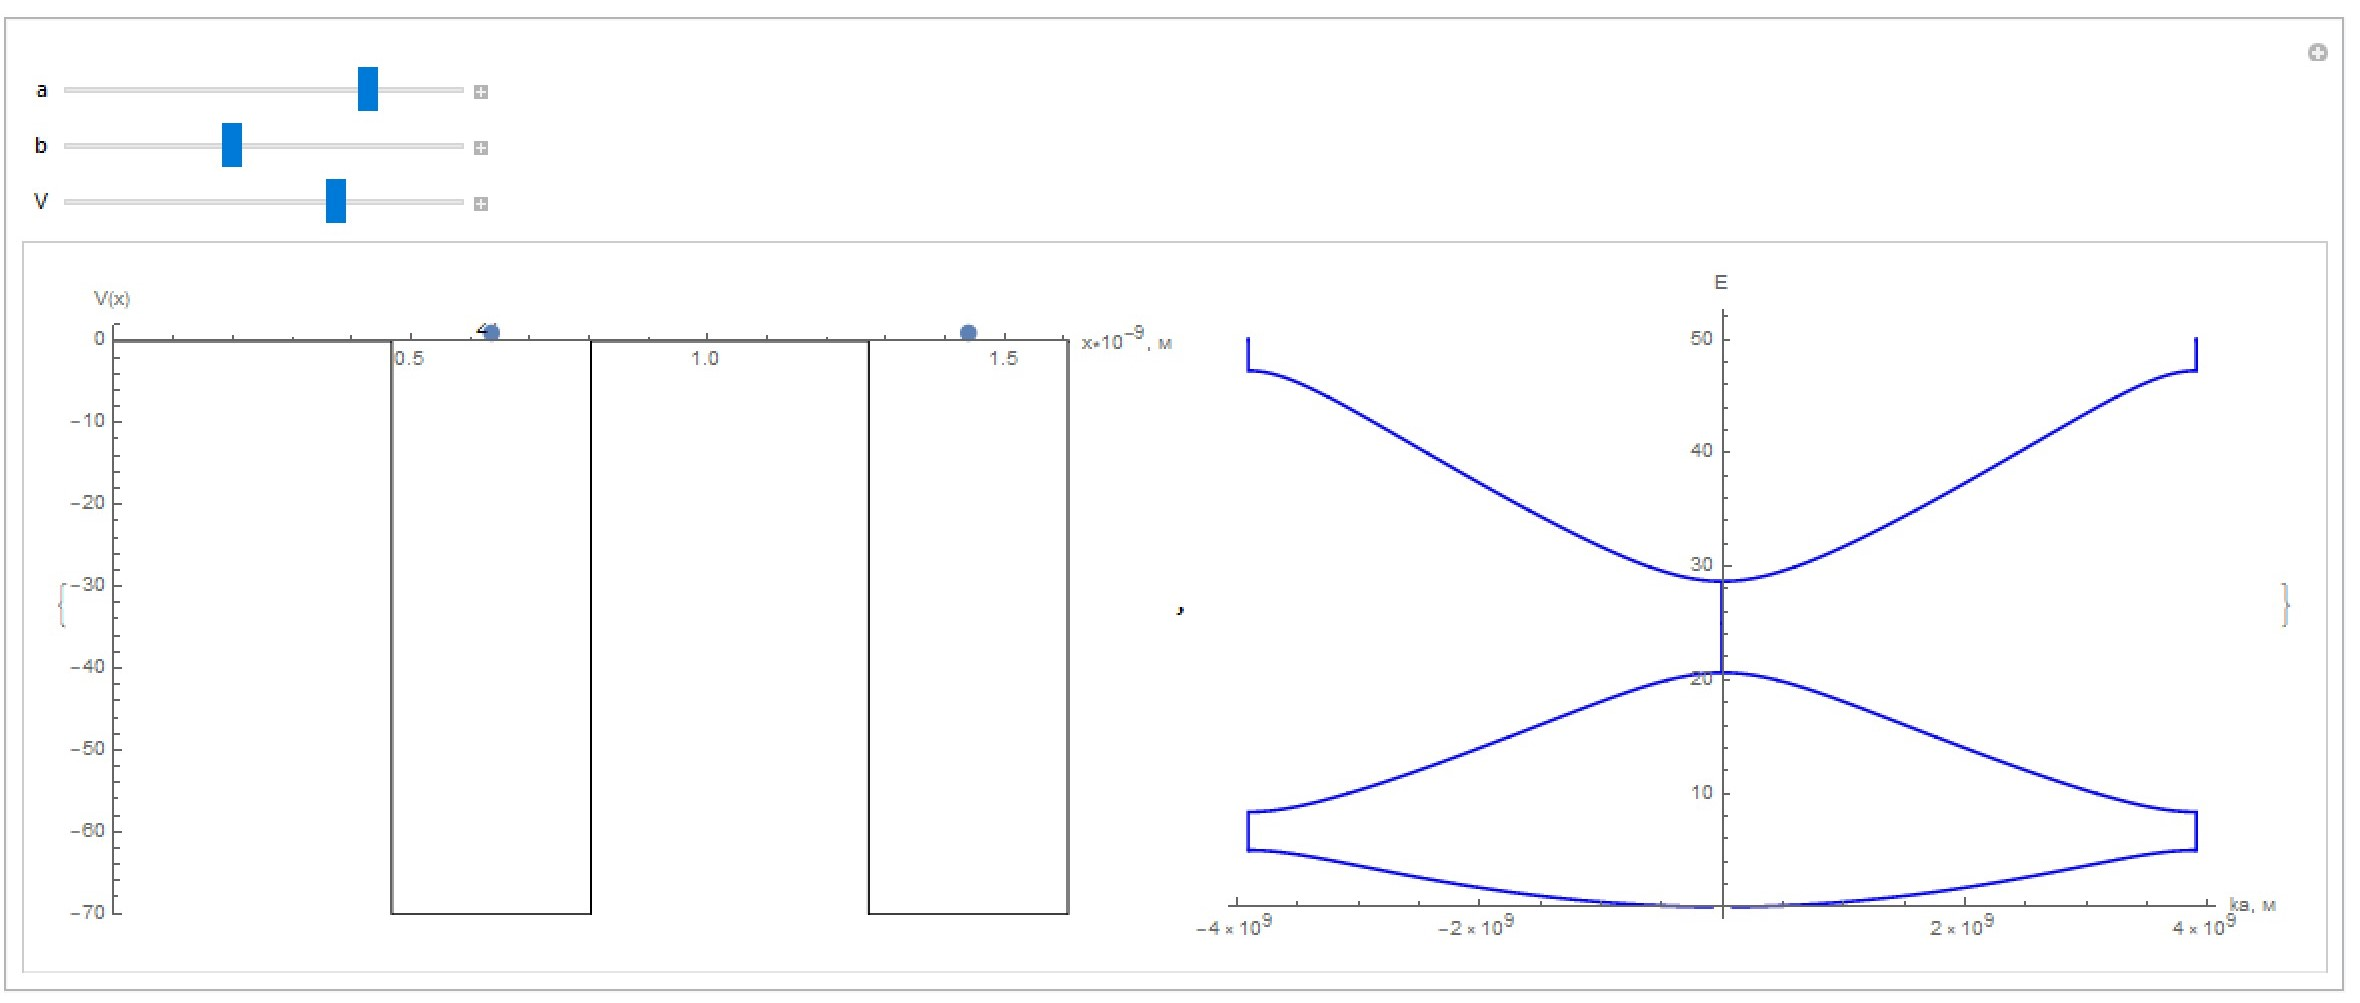
\includegraphics[width=\textwidth]{SharedScreenshot.jpg}
    \end{figure}
    \newpage
    \subsection{Зависимость ширины запрещенной зоны от ширины ямы}
    На основе полученного метода построим график зависимости ширины запрещенной зоны от ширины ямы при неизменных значениях её глубины и периоде потенциала. Расчет проведен для периода 10 $\angstrom$ и при глубине ямы $V_0=60$.
    \begin{figure}[!h]
        \centering
        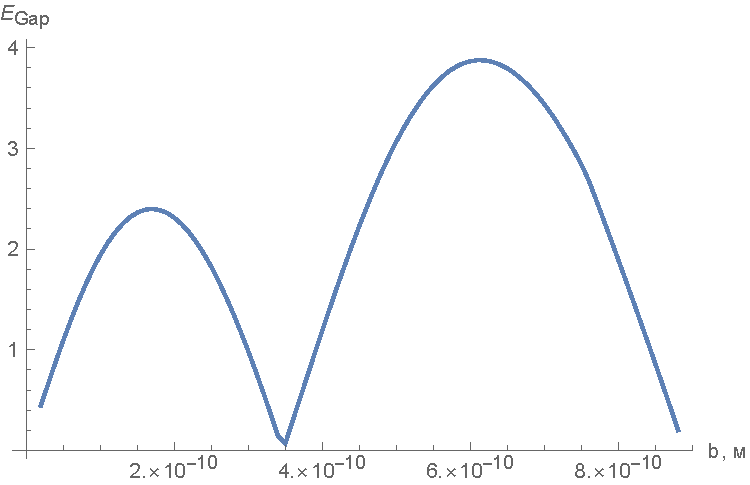
\includegraphics{bandGap.pdf}
        \caption{Ширина запрещенной зоны при периоде 10$\angstrom$ и глубине ямы $V_0=60$}
    \end{figure}

    \subsection{Зависимость ширины разрешенной зоны от ширины потенциальной ямы}
    Аналогичным методом можем получить вид зависимости ширины разрешенной зоны от ширины ямы:
    \begin{figure}[!h]
        \centering
        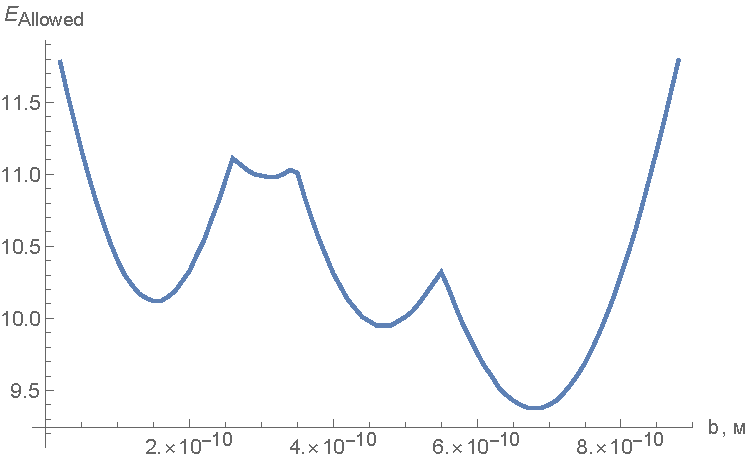
\includegraphics{allowedBand.pdf}
        \caption{Ширина разрешнной зоны при периоде 10$\angstrom$ и глубине ямы $V_0=60$}
    \end{figure}
\end{document}